% 	TOKAMAK
\begin{frame}
\frametitle{Tokamak}
\framesubtitle{}
\begin{columns}
	\begin{column}{0.4\textwidth}
		\begin{center}
		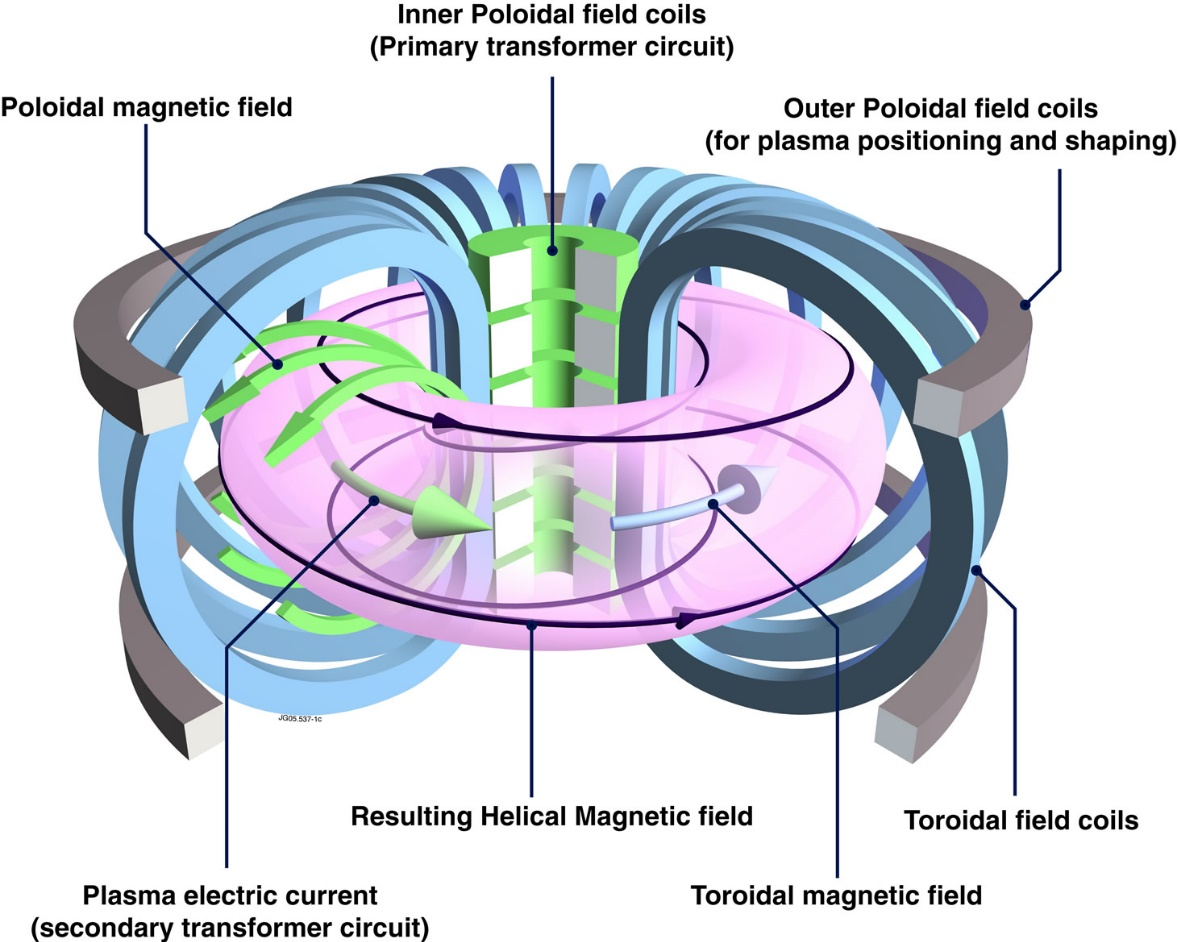
\includegraphics[scale=0.1]{Immagini/tokamak.png}
		\end{center}
		\begin{itemize}
			\item Superfici di campo chiuse, di forma toroidale
			\item Moti di deriva
		\end{itemize}
	\end{column}
	\begin{column}{0.4\textwidth}
		\begin{itemize}
			\item {\bf Plasma:} gas fortemente ionizzato
			\item {\bf Tokamak:} dispositivo toroidale
			\item {\bf Confinamento:} campi magnetici variabili
		\end{itemize}
		\begin{center}
		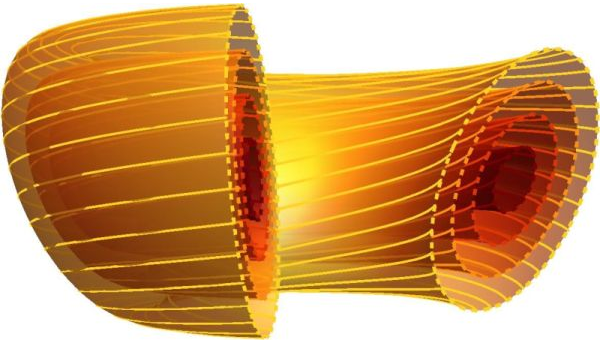
\includegraphics[scale=0.15]{Immagini/superfici.png}
		\end{center}
	\end{column}
\end{columns}
\end{frame}

% RISCALDAMENTO CON FASCIO
\begin{frame}
\frametitle{Neutral Beam Injection}
\begin{center}
\begin{itemize}
	\item Utile a riscaldare il plasma
	\item I neutri vengono ionizzati
	\item Prompt Losses
\end{itemize}
\end{center}
%{\bfseries Il flusso di particelle sulle pareti potrebbe danneggiare irreparabilmente il dispositivo.}
\end{frame}

% ELMs
\begin{frame}
\frametitle{ELMs}
\framesubtitle{Edge Localized Modes}
\begin{center}
\begin{itemize}
	\item Perturbazioni magnetoidrodinamiche al bordo del plasma
	\item Rilassamento del confinamento magnetico
	\item Due fasi: inter-ELM, intra-ELM
\end{itemize}
\end{center}
{\bfseries Il flusso di particelle sulle pareti potrebbe danneggiare irreparabilmente il dispositivo.}
\end{frame}



